\documentclass[a4paper,10pt]{article}

\usepackage[utf8]{inputenc}
\usepackage{epsfig}
\usepackage{amsmath}
\usepackage{amssymb}
\usepackage{array}
\usepackage{float} 
\usepackage{ctable}
\usepackage{multirow}
\usepackage{graphicx}
\usepackage{caption}
\usepackage{subcaption}
\usepackage{amsfonts}
\usepackage{cite}
\usepackage{algorithmic}


\def\th{^{th}}
\newcommand{\bs}[1]{\boldsymbol{#1}}



\title{Population Dynamics}
\author{Carlos Barreto}

\begin{document}

\maketitle







Revision protocols:

Each agent might have an opportunity to update its strategy (revision opportunity). The $i\th$ agent might compare the average profit of its strategy with the profit of other strategy. Then, might change its strategy with rate $\rho_{ij}$.

\subsection{Pairwise Proportional Imitation}

The $i\th$ agent observes an opponent $j$ at random. Then might change its strategy if  its opponent has a greater fitness. The rate change is 

\begin{equation}
\rho_{ij}(\pi, x) = \frac{x_j}{m} [\pi_j - \pi_i]_+
\end{equation}

In this case, $x_j$ need not be observed. 


	

\subsection{Comparison of the Average Payoff}

The $i\th$ agent selects a strategy at random and might switch to it if that strategy has payoff above the average. The agent switch strategy with probability proportional to the excess payoff

\begin{equation}
\rho_{ij}(\pi, x) = \left[ \pi_j - \frac{1}{m} \sum_{k\in S} x_k \pi_k \right]_+
\end{equation}



\subsection{Pairwise Comparison}

$i\th$ agent selects a strategy at random. If the opponent has a higher fitness, the the agent switch strategy with probability proportional to

\begin{equation}
\rho_{ij}(\pi, x) = \left[ \pi_j - \pi_i \right]_+
\end{equation}





\subsection{Logit Choice}

The $i\th$ agent selects a strategy at random and change its strategy with a probability proportional to 

\begin{equation}
\rho_{ij}(\pi) = \frac{ \exp(\pi_j \eta^{-1} ) }{ \sum_{k \in S} \exp(\pi_k \eta^{-1} ) }
\end{equation}









\subsection{Evolutionary Dynamics} \label{sec:dynamics}

We implement four evolutionary dynamics, namely \emph{logit dynamics} (Logit), \emph{replicator dynamics} (RD), \emph{Brown-von Neumann-Nash dynamics} (BNN), and \emph{Smith dynamics} (Smith) that belong to the families of \emph{perturbed optimization}, \emph{imitative dynamics}, \emph{excess payoff dynamics}, and \emph{pairwise comparison dynamics}, respectively \cite{hofbauer2001nash, sandholm_book}. 
%
%
Each family uses different agent behavior models. A priori, it is difficult to know which dynamic is most convenient for a particular problem. 
Now, let us denote the dynamics of a society by means of 
%
\begin{equation}
\dot{ \bs{x} } = V_d( \bs{x} ),
\end{equation}
where $d\in \mathcal{D}=\{ Logit, RD, Smith, BNN \}$ denotes the dynamic used.
The following differential equations describe the evolution in time of each strategy according to each evolutionary dynamic:
%
\subsubsection{Logit Dynamics}
\begin{equation}\label{eq:logit}
 \dot{x}_k^i = \frac{ \exp\left(\eta^{-1} F_k^i (\bs{x}) \right) }{ \sum_{\gamma \in S} \exp\left(\eta^{-1} F_\gamma^i (\bs{x}) \right) }, \, \, \eta>0,
\end{equation}

\subsubsection{Replicator Dynamics}
\begin{equation}\label{eq:replicator}
\dot{x}_k^i = x_k^i \, \hat{F}_k^i \left( \bs{x} \right).
\end{equation}

\subsubsection{Brown-von Neumann-Nash Dynamics (BNN)}
\begin{equation}\label{eq:bnn}
 \dot{x}_k^i = \left[ \hat{F}_k^i \left( \bs{x} \right) \right]_+ - x_k^i  \sum_{\gamma \in S} \left[ \hat{F}_\gamma^i \left( \bs{x} \right) \right]_+
\end{equation}

\subsubsection{Smith Dynamics}
\begin{multline}
\dot{x}_k^i  = \sum_{\gamma \in S} x_\gamma^i  \left[ F_k^i \left( \bs{x} \right) - F_\gamma^i \left( \bs{x} \right) \right]_+ 
\\
- x_k^i  \sum_{\gamma \in S} \left[ F_\gamma^i ( \bs{x}) - F_k^i( \bs{x} ) \right]_+.
\label{eq:smith}
\end{multline}



These dynamics are defined in function of the excess payoff to strategy $k$ as $\hat{F}_k^i =  F_k^i(\bs{q}^k) - \bar{F}_k^i(\bs{q}^k)$,
where $\bar{F}_k^i(\bs{q}^k)$ is the average payoff the population $i$.







\subsection{Maynard Smith Replicator}

\begin{equation}
\dot{x}_i = \frac{ x_i F_i }{ \bar{F}(x) } - x_i
\end{equation}






\section{Examples}
We show examples of two games that have different number of populations and strategies per population.

\subsection{Rock-paper-scissors game}
We implement the rock-paper-scissors game. This game has only one population with three strategies, denoted $x = [x_1, x_2, x_3]^\top$. The fitness function is defiined as $F(x)=Ax$, where A is equal to 
\begin{equation}
  A = \begin{pmatrix}
  0  & -1 &  1 \\
  1  &  0 & -1 \\
  -1 &  1 & 0
  \end{pmatrix}
\end{equation}


\begin{figure}
  \centering
  \begin{subfigure}[b]{0.45\textwidth}
	  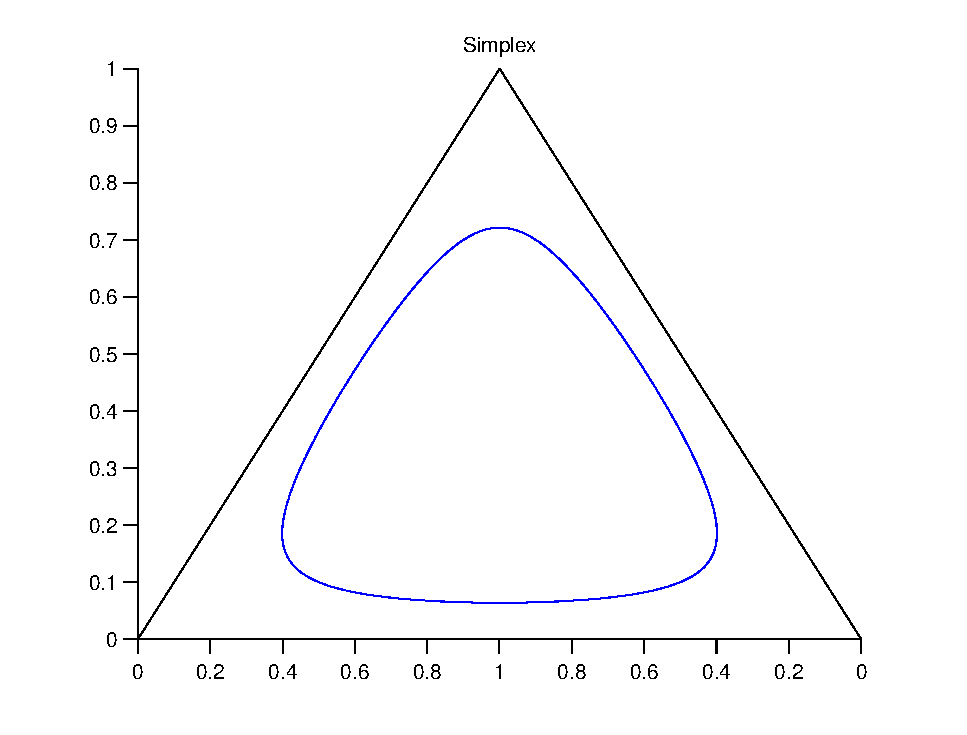
\includegraphics[width=\textwidth]{./images/test1_simplex_rd.eps}
	  \caption{Simplex.}
	  \label{fig:test1_simplex_rd}
  \end{subfigure}
  ~ 
  \begin{subfigure}[b]{0.45\textwidth}
	  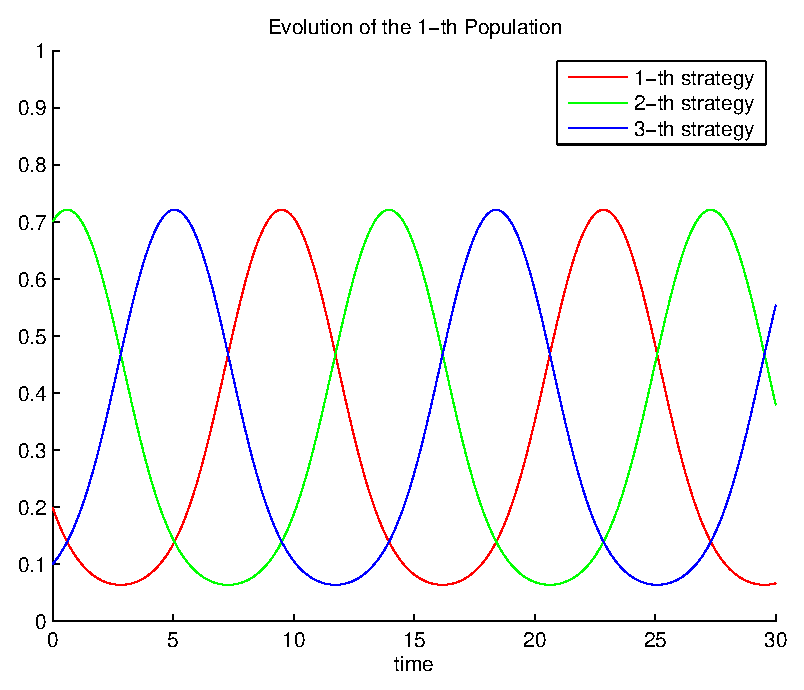
\includegraphics[width=\textwidth]{./images/test1_ev_rd.eps}
	  \caption{Evolution of the strategies in time.}
	  \label{fig:test1_ev_rd}
  \end{subfigure}
  \caption{Rock-paper-scissors game with replicator dynamics.}
  \label{fig:rpc_game_rd}
\end{figure}


\begin{figure}
  \centering
  \begin{subfigure}[b]{0.45\textwidth}
	  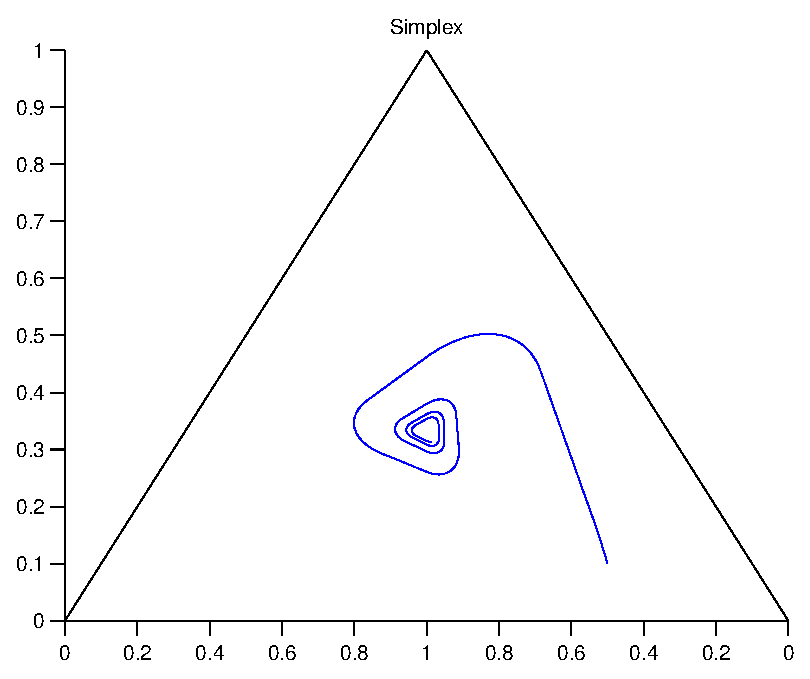
\includegraphics[width=\textwidth]{./images/test1_simplex_bnn.eps}
	  \caption{Simplex.}
	  \label{fig:test1_simplex_bnn}
  \end{subfigure}
  ~ 
  \begin{subfigure}[b]{0.45\textwidth}
	  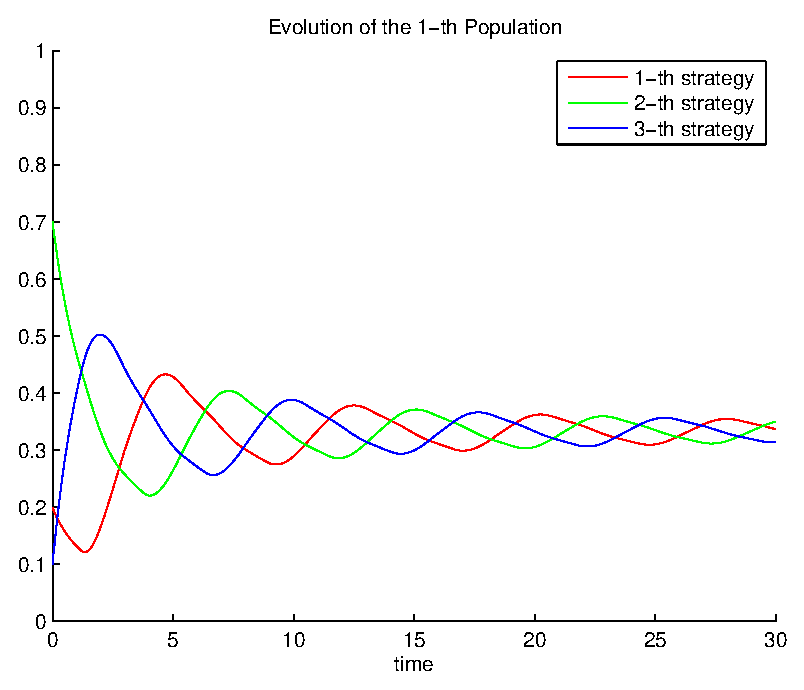
\includegraphics[width=\textwidth]{./images/test1_ev_bnn.eps}
	  \caption{Evolution of the strategies in time.}
	  \label{fig:test1_ev_bnn}
  \end{subfigure}
  \caption{Rock-paper-scissors game with BNN dynamics.}
  \label{fig:rpc_game_bnn}
\end{figure}



\begin{figure}
  \centering
  \begin{subfigure}[b]{0.45\textwidth}
	  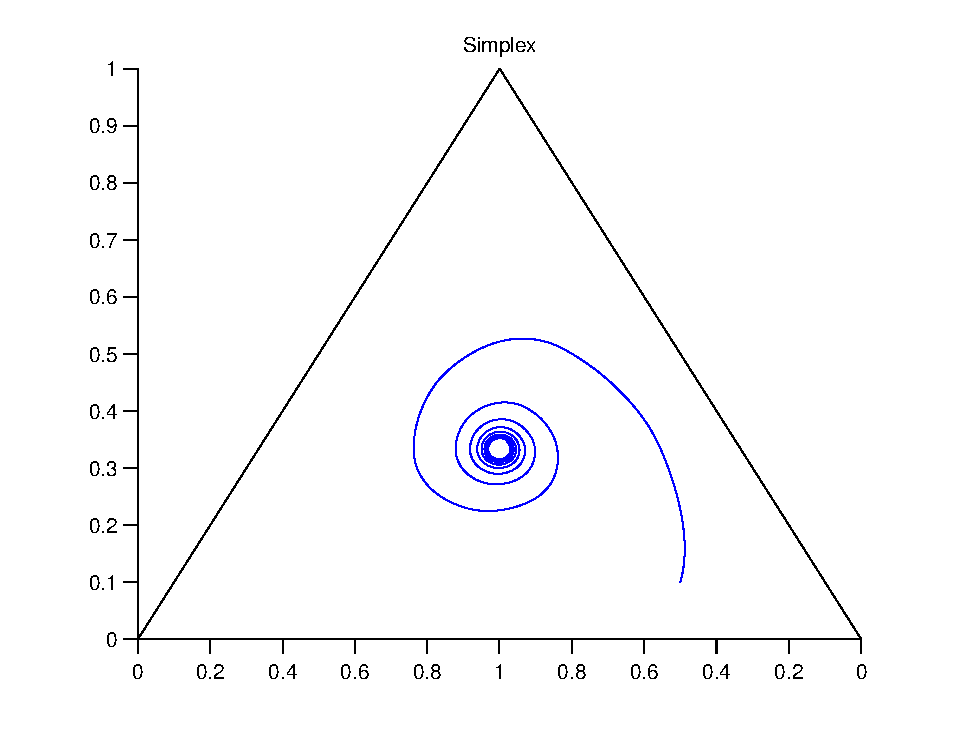
\includegraphics[width=\textwidth]{./images/test1_simplex_smith.eps}
	  \caption{Simplex.}
	  \label{fig:test1_simplex_smith}
  \end{subfigure}
  ~ 
  \begin{subfigure}[b]{0.45\textwidth}
	  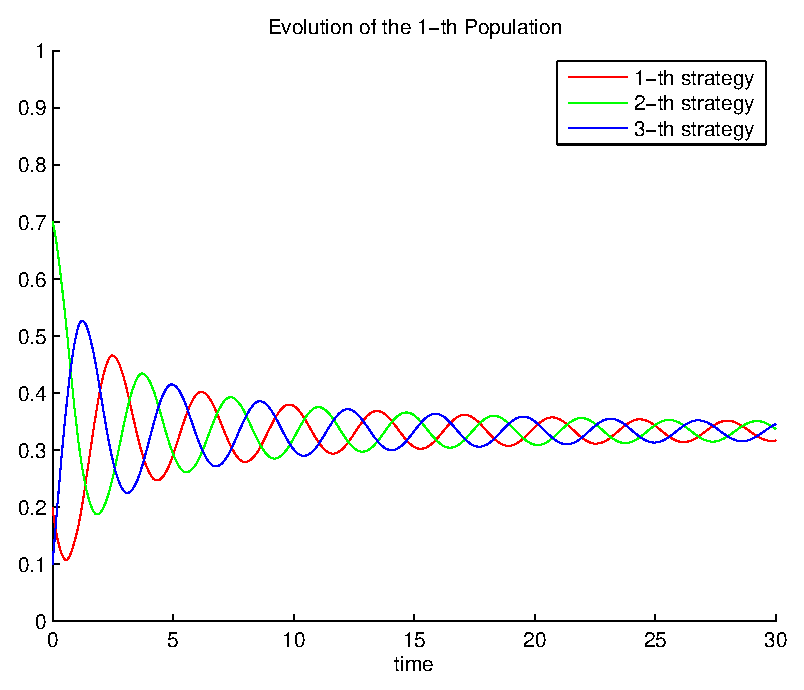
\includegraphics[width=\textwidth]{./images/test1_ev_smith.eps}
	  \caption{Evolution of the strategies in time.}
	  \label{fig:test1_ev_smith}
  \end{subfigure}
  \caption{Rock-paper-scissors game with Smith dynamics.}
  \label{fig:rpc_game_smith}
\end{figure}



\begin{figure}
  \centering
  \begin{subfigure}[b]{0.45\textwidth}
	  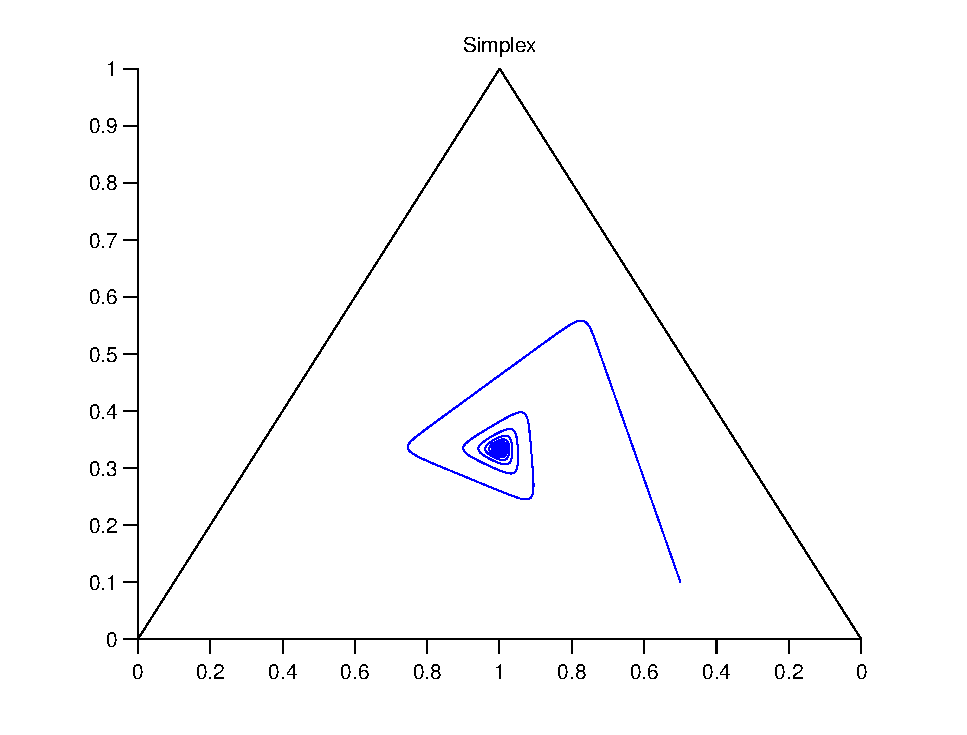
\includegraphics[width=\textwidth]{./images/test1_simplex_logit.eps}
	  \caption{Simplex.}
	  \label{fig:test1_simplex_logit}
  \end{subfigure}
  ~ 
  \begin{subfigure}[b]{0.45\textwidth}
	  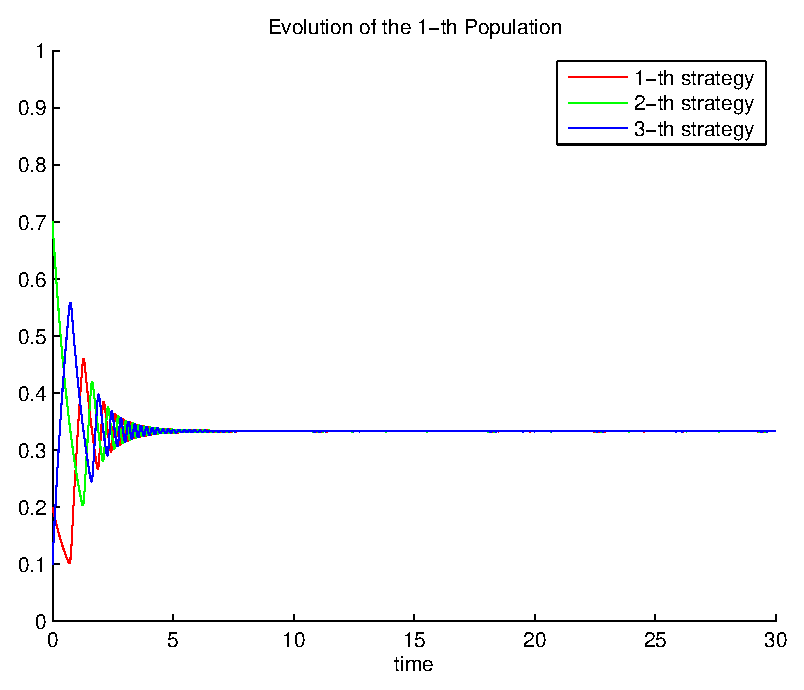
\includegraphics[width=\textwidth]{./images/test1_ev_logit.eps}
	  \caption{Evolution of the strategies in time.}
	  \label{fig:test1_ev_logit}
  \end{subfigure}
  \caption{Rock-paper-scissors game with logit dynamics.}
  \label{fig:rpc_game_logit}
\end{figure}





\subsection{Matching pennies}
We implement a matching pennies game with two populations. First, note that the payoff of the game in normal form is
%
\begin{table}[h]
\centering
 \begin{tabular}{|c|c|} \hline
  2, 1 & 1, 2 \\ \hline
  1, 2 & 2, 1 \\ \hline
 \end{tabular}
\end{table}
%
In this case each population has two strategies, namely \emph{heads} and \emph{tails}.
Now, the fitness of the $i^{th}$ population can be expressed as $F^i(x^i) = A_i x^i$, for $i=\{x_h^i, x_t^i\}$. 
The payoff matrices are defines as follows
%
\begin{equation}
  A_1 = \begin{pmatrix}
2 & 1 \\
1 & 2 
  \end{pmatrix}
\end{equation}
%
\begin{equation}
  A_2 = \begin{pmatrix}
  1 & 2 \\
  2 & 1 
  \end{pmatrix}
\end{equation}
%


\begin{figure}
  \centering
  \begin{subfigure}[b]{0.45\textwidth}
	  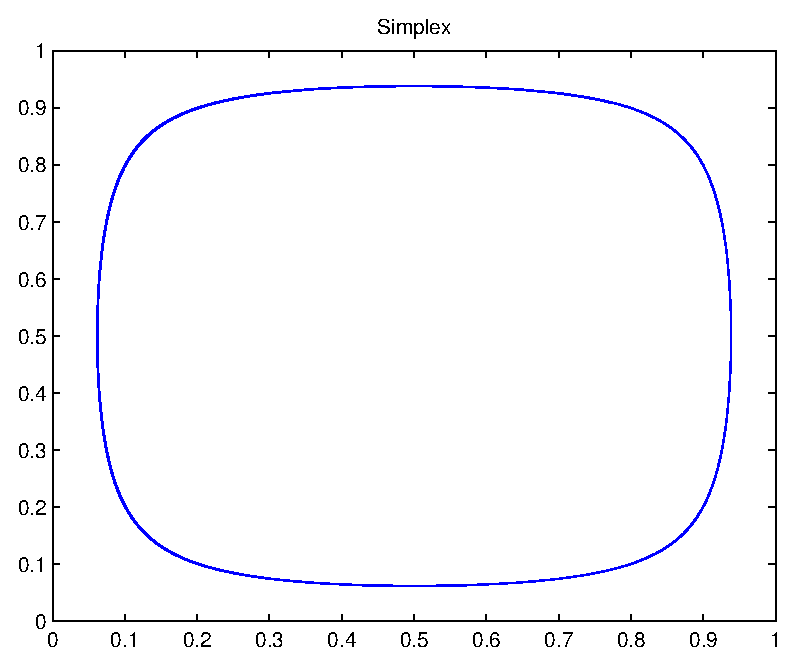
\includegraphics[width=\textwidth]{./images/test2_simplex_rd.eps}
	  \caption{Simplex.}
	  \label{fig:test2_simplex_rd}
  \end{subfigure}
  ~ 
  \begin{subfigure}[b]{0.45\textwidth}
	  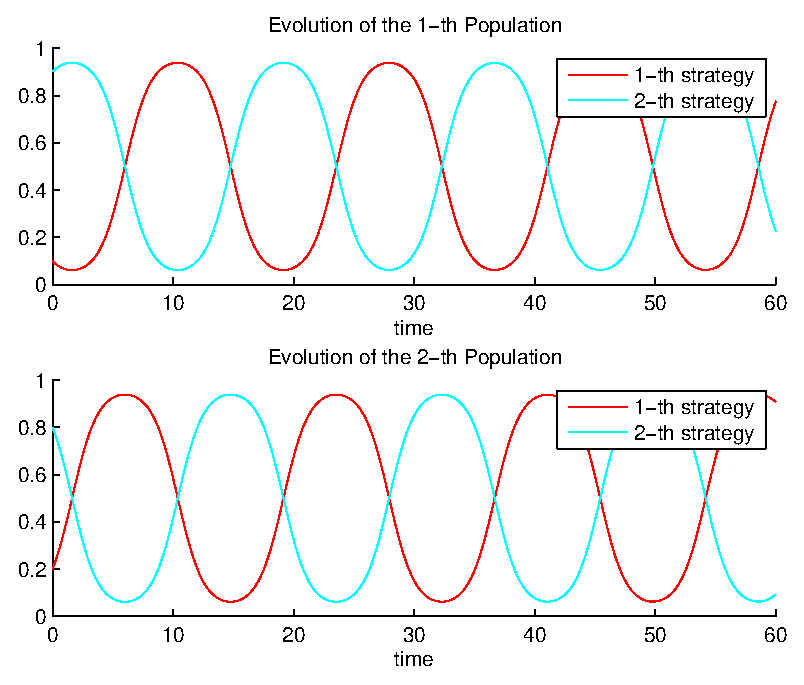
\includegraphics[width=\textwidth]{./images/test2_ev_rd.eps}
	  \caption{Evolution of the strategies in time.}
	  \label{fig:test2_ev_rd}
  \end{subfigure}
  \caption{Matching pennies game with replicator dynamics.}
  \label{fig:mp_game_rd}
\end{figure}


\begin{figure}
  \centering
  \begin{subfigure}[b]{0.45\textwidth}
	  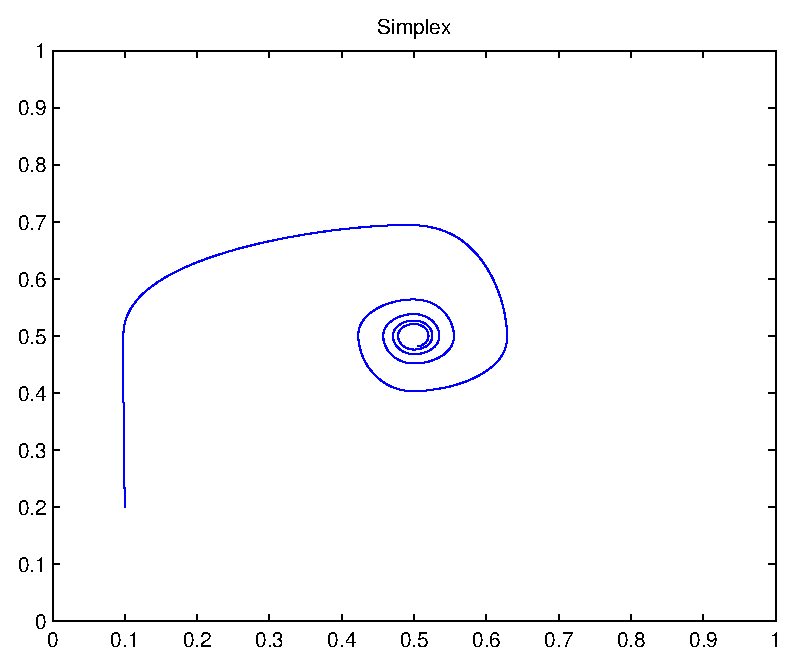
\includegraphics[width=\textwidth]{./images/test2_simplex_bnn.eps}
	  \caption{Simplex.}
	  \label{fig:test2_simplex_bnn}
  \end{subfigure}
  ~ 
  \begin{subfigure}[b]{0.45\textwidth}
	  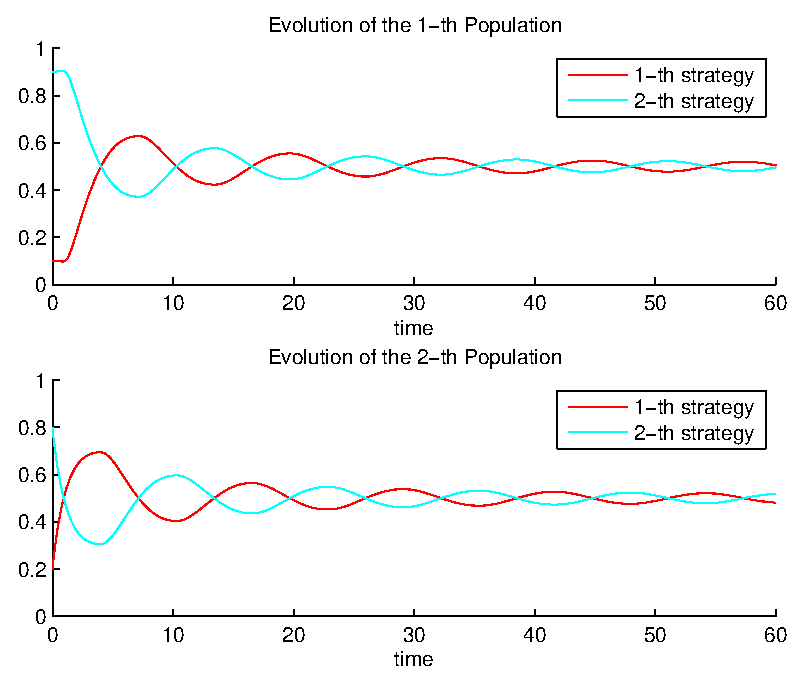
\includegraphics[width=\textwidth]{./images/test2_ev_bnn.eps}
	  \caption{Evolution of the strategies in time.}
	  \label{fig:test2_ev_bnn}
  \end{subfigure}
  \caption{Matching pennies game with BNN dynamics.}
  \label{fig:mp_game_bnn}
\end{figure}



\begin{figure}
  \centering
  \begin{subfigure}[b]{0.45\textwidth}
	  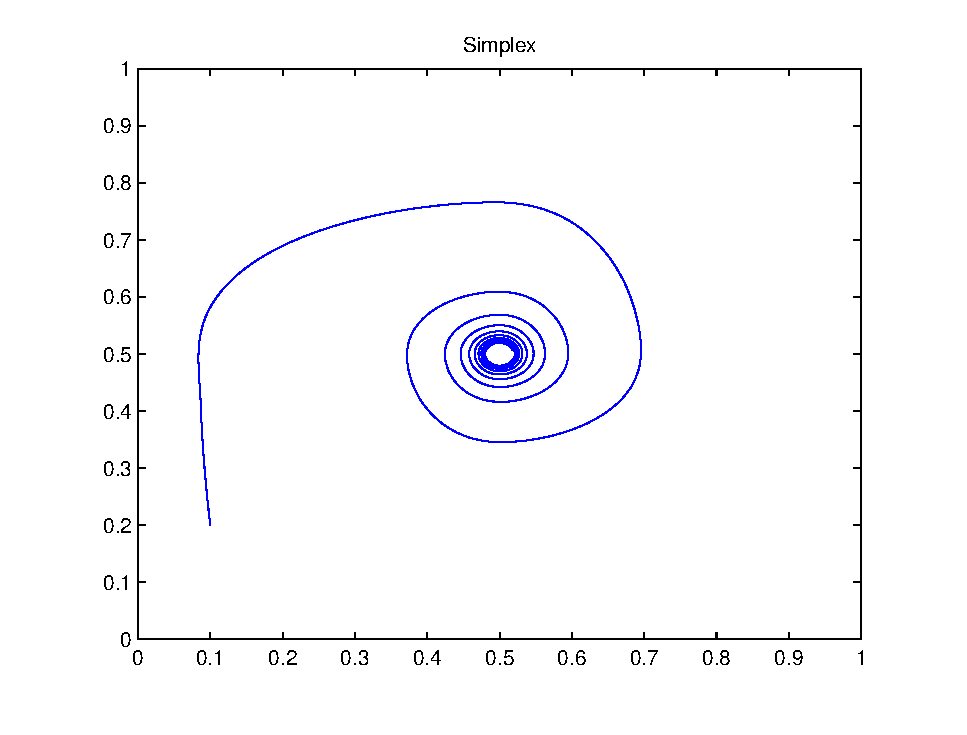
\includegraphics[width=\textwidth]{./images/test2_simplex_smith.eps}
	  \caption{Simplex.}
	  \label{fig:test2_simplex_smith}
  \end{subfigure}
  ~ 
  \begin{subfigure}[b]{0.45\textwidth}
	  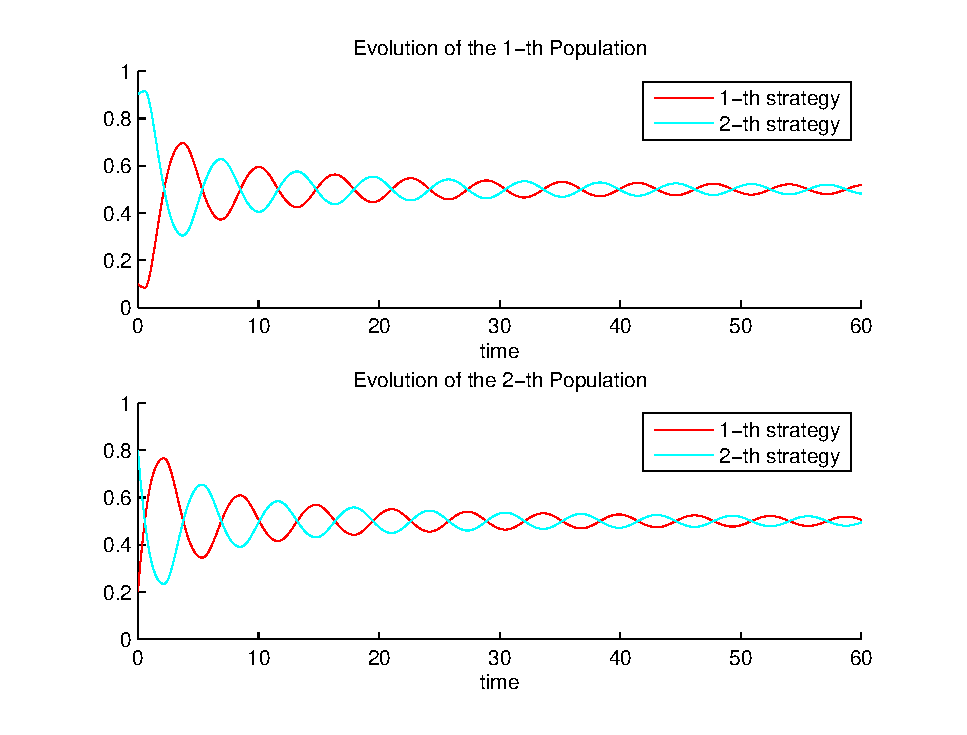
\includegraphics[width=\textwidth]{./images/test2_ev_smith.eps}
	  \caption{Evolution of the strategies in time.}
	  \label{fig:test2_ev_smith}
  \end{subfigure}
  \caption{Matching pennies game with Smith dynamics.}
  \label{fig:mp_game_smith}
\end{figure}



\begin{figure}
  \centering
  \begin{subfigure}[b]{0.45\textwidth}
	  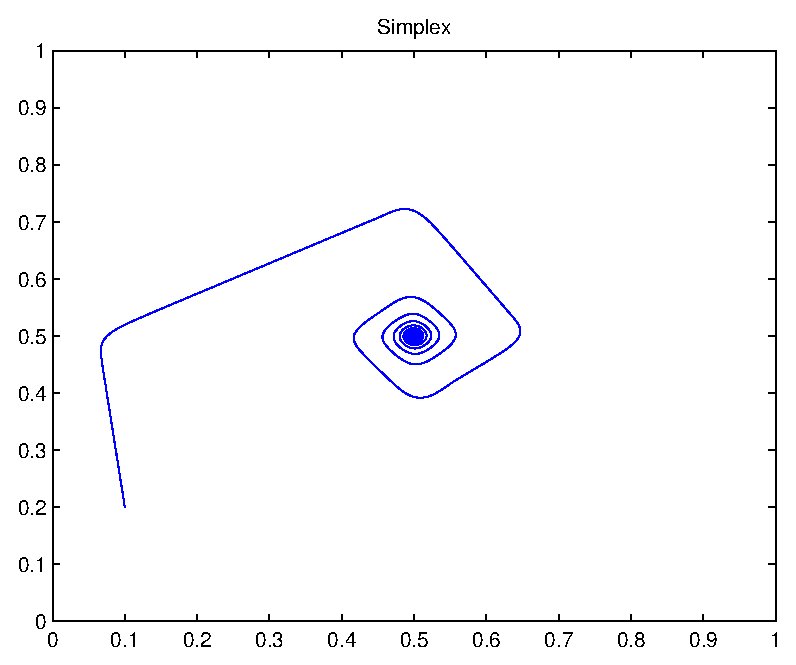
\includegraphics[width=\textwidth]{./images/test2_simplex_logit.eps}
	  \caption{Simplex.}
	  \label{fig:test2_simplex_logit}
  \end{subfigure}
  ~ 
  \begin{subfigure}[b]{0.45\textwidth}
	  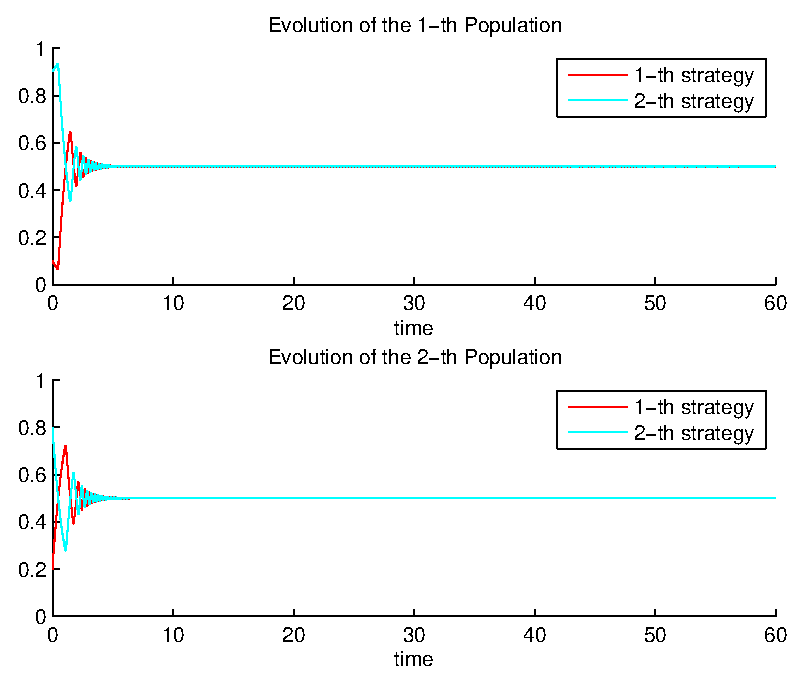
\includegraphics[width=\textwidth]{./images/test2_ev_logit.eps}
	  \caption{Evolution of the strategies in time.}
	  \label{fig:test2_ev_logit}
  \end{subfigure}
  \caption{Matching pennies game with logit dynamics.}
  \label{fig:mp_game_logit}
\end{figure}










\section{Designing games}

In the previous section we show some examples of strategical situations that can be analyzed with game theory. In these cases, the structure of the game is given by the problem. However, we can modify the fitness function of each player in order to solve an optimization problem.

For example, let us consider the following optimization problem:

\begin{equation}\label{eq:opt_problem}
\begin{aligned}
& \underset{x}{\text{maximize}} 
& & \sum_{i=1}^N U_i(x_i)  - C(|x|)\\
& \text{subject to}
& & 0 \leq q_i \geq m,  i =\{1,\ldots, N\}.
\end{aligned}
\end{equation}

This can be seen as a problem of allocating a finite resource to maximize a utility function. 

Note that there are $N$ agents with that give a valuation $v_i(x_i)$ to the resource $x_i$.

However, the cost of assigning the resource is $C(|x|)$ .

The cost of assigning the resource might be distributed among the population. 

Let us consider the following example:


\begin{equation}
U_i(x_i) =   \alpha_i  log(1+x_i) 
\end{equation}

\begin{equation}
C(z) = \beta z^2 + b z 
\end{equation}

define fitness functions as 

\begin{equation}
f_i(x_1, x_2) = \frac{\alpha_i}{1+x_i} - 2 \beta |x| - b 
\end{equation}











\section{Finite time}


The continuous dynamics are based on two assumptions, namely, myopia and inertia. 

Inertia: agents do not reevaluate their actions continuously. They reevaluate their decisions at ramdom time stamps.

The evolution might take place in days, months, years.

Myopia means that agents determine their future actions according to the current bahavior of other agents as well as the expected payoff in the current state. This is assumed in contexts where the population state do not change fast.


------------

With a finite population the time specifies the number of iterations.

There might be different populations!!!

How do we define the state vector???


\iffalse


      
\begin{figure}[htb]
 \includegraphics[1\textwidth]{./images/}
 \caption{}
 \label{fig:}
\end{figure}




test1_ev_bnn.eps         test1_simplex_rd.eps     test2_simplex_bnn.eps
test1_ev_logit.eps       test1_simplex_smith.eps  test2_simplex_logit.eps
test1_ev_rd.eps          test2_ev_bnn.eps         test2_simplex_rd.eps
test1_ev_smith.eps       test2_ev_logit.eps       test2_simplex_smith.eps
test1_simplex_bnn.eps    test2_ev_rd.eps
test1_simplex_logit.eps  test2_ev_smith.eps
\fi

\end{document}
